% todo: modificare l'immagine sopra ad "anatomical surrogate generation" con uno screen di ParaView.
% todo: aggiungere immagini sopra al branch del modello meccanico.

\begin{figure}[H]\centering
  \begin{tikzpicture}[node distance=3cm]
    % Nodes
    %% Chaste & Morphometric Model
    \node (ct_acquisition)           [startstop] {CT\\Acquisition};
    % \node (img_ct_acquisition)       [image, above of=ct_acquisition, yshift=-1.0cm]                   {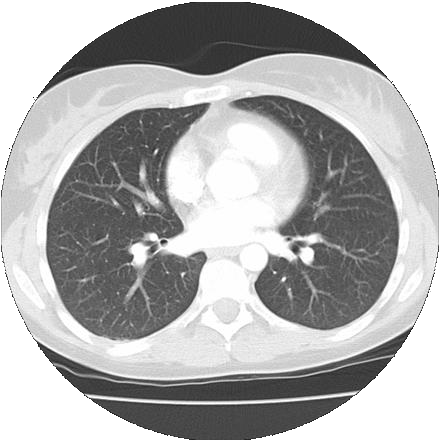
\includegraphics[width=2.0cm]{ct_acquisition.png}};
    %%% Upper branch
    \node (lobes_segmentation)       [process, right of=ct_acquisition, xshift=3.25cm, yshift=+2cm]    {Lobes\\segmentation};
    %%% Lower branch
    % \node (img_lobes_segmentation)   [image, above of=lobes_segmentation, xshift=-.1cm, yshift=-1.2cm] {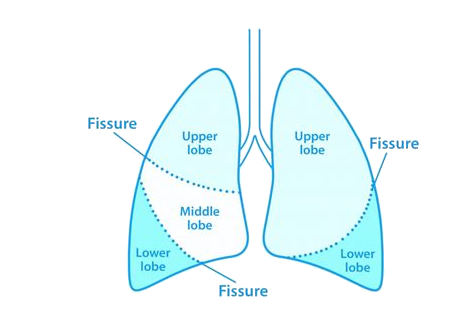
\includegraphics[width=3.5cm]{lobes_segmentation.png}};
    \node (airways_segmentation)     [process, below of=lobes_segmentation, xshift=-2cm, yshift=-1cm]  {Airways\\segmentation};
    % \node (img_airways_segmentation) [image, above of=airways_segmentation, xshift=2cm, yshift=-1cm]   {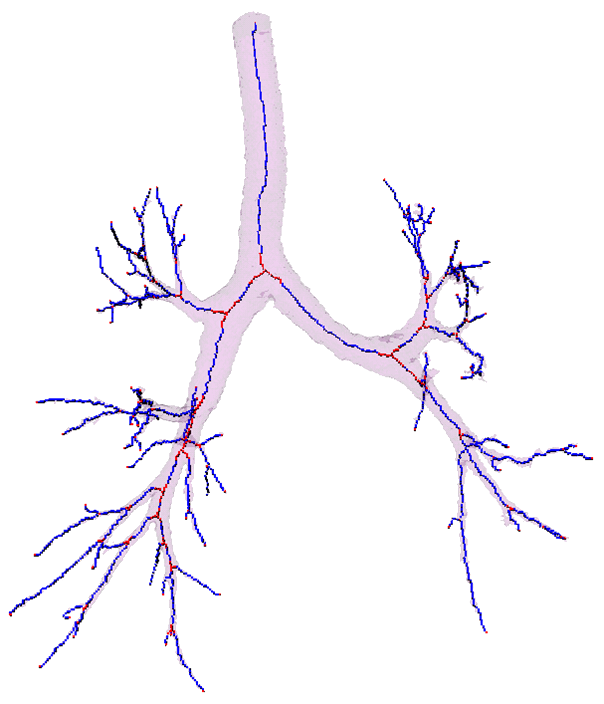
\includegraphics[height=2.5cm]{airways_segmentation.png}};
    \node (centerline_extraction)    [process, below of=lobes_segmentation, xshift=+2cm, yshift=-1cm]  {Centerline\\extraction};
    \node (surrogate_generation)     [process, right of=ct_acquisition, xshift=9.5cm]                  {Anatomical surrogate\\generation};
    % \node (img_surrogate_generation) [image, above of=surrogate_generation, yshift=-.5cm]              {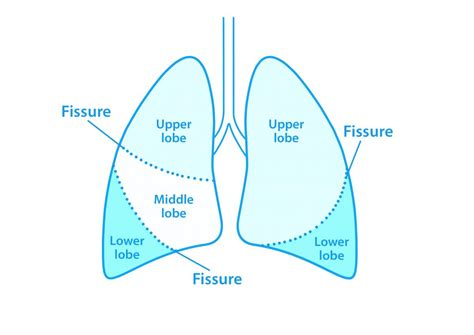
\includegraphics[width=3.5cm]{lobes_segmentation.jpg}};
    %% Julia & Mechanical Model
    \node (parameters_update)        [process, below of=ct_acquisition, yshift=-2cm]                   {Lungs parameters\\update};
    \node (model_instantiation)      [process, right of=parameters_update, xshift=1cm]                 {Mechanical model\\instantiation};
    \node (DAE_solution)             [process, right of=model_instantiation, xshift=1cm]               {DAE System\\solution};
    \node (simulations)              [startstop, right of=DAE_solution, xshift=+1cm]                   {Mechanical Simulations};

    % Arrows
    \draw [arrow] (ct_acquisition.east)                              -- ++(.5,0) coordinate(tmp)     |- (airways_segmentation.west);
    \draw [arrow] (airways_segmentation)                             -- (centerline_extraction);
    \draw [arrow] (centerline_extraction.east)                       -- ++(.5,0) coordinate(tmp1)    |- (surrogate_generation.west);
    \draw [arrow] (model_instantiation)                              -- (DAE_solution);
    \draw [arrow] (DAE_solution)                                     -- (simulations);
    \draw [arrow] (tmp)                                              |-   (lobes_segmentation.west);
    \draw [arrow] (lobes_segmentation)                               --   (tmp1|-lobes_segmentation) |- (surrogate_generation.west);
    \draw [dashed, thick, ->,>=stealth] (surrogate_generation.south) -- ++(0,-2.5)                   -| (parameters_update.north);
    \draw [arrow] (parameters_update)                                -- (model_instantiation);

    % Frame around a part of the flowchart
    \begin{pgfonlayer}{background}
      \node[rounded corners=3mm,
      draw=blue,
      thick, dashed,
      % fit=(airways_segmentation)(centerline_extraction)(img_lobes_segmentation)(img_surrogate_generation),
      fit=(airways_segmentation)(centerline_extraction)(lobes_segmentation)(surrogate_generation),
      fill=cyan!5,
      inner sep=7pt,
      label={[anchor=south]above:\textsc{\textcolor{blue}{Morphometric model}}}] {};
    \end{pgfonlayer}
    \begin{pgfonlayer}{background}
      \node[rounded corners=3mm,
      draw=red,
      thick, dashed,
      fit=(parameters_update)(model_instantiation)(DAE_solution),
      fill=magenta!5,
      inner sep=7pt,
      label={[anchor=south]above:\textsc{\textcolor{red}{Mechanical model}}}] {};
    \end{pgfonlayer}
  \end{tikzpicture}
  \caption{Data pipeline.  The process begins with a
    \emph{patient-specific image} (i.e. CT) of a premature newborn.
    The extracted data, comprising \emph{two segmentations}, are then
    processed to obtain an anatomical surrogate of the airway tree.
    This is necessary due to scanner resolution not allowing for the
    discrimination and localization of small branches.  From the
    resulting morphometric model, the \emph{mechanical parameters} can
    be derived, which are essential for generating an accurate
    simulation model.  Finally, a numerical solver for differential
    equations provides the final output.}
    \label{fig:data_pipeline}
\end{figure}

%%% Local Variables:
%%% mode: LaTeX
%%% TeX-master: "../Thesis"
%%% End:
